 \documentclass{article}
\usepackage[utf8]{inputenc}
\usepackage{polski}
\usepackage[T1]{fontenc}
\usepackage{amsmath,amssymb,amsthm}
\usepackage{lmodern}
\usepackage{geometry}
\usepackage[dvipsnames]{xcolor}
\usepackage{hyperref}
\usepackage{array}
\usepackage{caption}
\usepackage{graphicx}

\newcommand{\plotskala}{0.45}

\newtheorem{tw}{Twierdzenie}[section]
\newtheorem{lem}{Lemat}[section]

\theoremstyle{definition}
\newtheorem{fa}[tw]{Fakt}

\begin{document}

\begin{center}
    \LARGE
    \textbf{Pracownia z Analizy numerycznej (M)}

    \medskip

    Sprawozdanie do zadania {\bf P2.1}

    \bigskip

    {\Large Jadwiga Świerczyńska}
    
    {\Large Wrocław, 05.01.2023 r.}
    
\end{center}

\vspace{70pt}

% ----------------------------------------------------------------------
% ---------------------------- WSTĘP -----------------------------------
% ----------------------------------------------------------------------

\section{Wstęp}

Całkowanie numeryczne (nazywane inaczej {\it kwadraturą}) to przybliżone obliczanie wartości całek oznaczonych. Dla wielu funkcji obliczenie dokładnej postaci całki nieoznaczonej jest zadaniem skomplikowanym. Wobec tego stosujemy metody numeryczne umożliwiające poznanie aproksymacji wartości całki. 

\medskip

\noindent Jedną z metod całkowania numerycznego jest kwadratura interpolacyjna. Interpolacja wielomianowa pozwala na przybliżanie funkcji poprzez wielomian w zadanych punktach. Całka z wielomianu interpolacyjnego jest więc przybliżeniem całki z danej funkcji. 

\medskip

\noindent Wzory na kwadraturę interpolacyjną są różne w zależności od doboru węzłów interpolacji. W poniższej pracy zbadano kwadraturę Newtona--Cotesa, w której węzły są równoodległe. W szczególności opisano wzory na tę metodę z dwoma węzłami ({\it wzór trapezów}), trzema ({\it wzór Simpsona}), a także z \(n\) węzłami. Ponadto wyprowadzono wzory na kwadratury złożone wykorzystujące {\it wzór trapezów} oraz {\it wzór Simpsona}. 

\medskip

\noindent W rozdziale \ref{roz:eksperymenty} opisano eksperymenty polegające na zastosowaniu kwadratury Newtona--Cotesa do różnych typów funkcji oraz porównano ich wyniki z wartościami zwracanymi przez funkcję \verb|quadgk| z biblioteki \verb|QuadGK.jl| z języka \verb|Julia|, które przyjęto jako wartości dokładne. 

\medskip

\noindent W rozdziale \ref{roz:czas} opisano, jak dokładne wyniki można osiągnąć, wykorzystując metodę trapezów i metodę Simpsona przy obliczeniach trwających nie dłużej niż \(0,001\) sekundy.

\newpage

% ----------------------------------------------------------------------
% ---------------------------- OPIS METODY------------------------------
% ----------------------------------------------------------------------

\section{Opis metody Newtona--Cotesa}

Metoda Newtona--Cotesa jest kwadraturą numeryczną wykorzystującą węzły równoodległe. Przypomnijmy sobie zatem wzór interpolacyjny Lagrange'a. 

\begin{fa}[Wzór interpolacyjny Lagrange'a]
    \label{wzor_interpolacyjny_Largange}
    Niech \(f(x)\) będzie funkcją określoną na \([a,b]\) oraz niech \(a \leq x_0, x_1, \ldots, x_n \leq b\) i \(x_i \neq x_j\) dla \(i \neq j\). Określmy
    \[
        \lambda_k(x) = \prod_{j=0, j \neq k}^{n} \frac{x-x_j}{x_k - x_j} \text{.}
    \]
    Wówczas wielomian
    \[
        L_n(x) = \sum_{k=0}^{n} f(x_k)\lambda_k(x)
    \]
    spełnia 
    \[
        L_n(x_i) = f(x_i) \text{ \hspace{10pt} dla \(i = 0, 1, \ldots, n\).}
    \]
\end{fa}

% \begin{fa}
%     \label{lambda_Largange_rownoodlegle}
%     Gdy \(x_i = a + ih\) dla \(h = \frac{b-a}{n}\) oraz \(i = 0, 1, \ldots, n\), to funkcja \(\lambda_k\) we wzorze interpolacyjnym Lagrange'a wyraża się wzorem
%     \[
%         \lambda_k(x) = \lambda_k\left( a + h\frac{x-a}{h} \right) = \prod_{j=0, j \neq k}^{n} \frac{\frac{x-a}{h} - j}{k - j} \text{.}
%     \]
% \end{fa}


\noindent Wartość całki z funkcji \(f\) możemy przybliżać wartością całki z wielomianu \(L_n\), czyli
\[
    \int_a^b f(x) \,dx \approx \int_a^b L_n(x) \,dx \text{.}
\]

\noindent Wyprowadźmy dokładny wzór na \(\int_a^b L_n(x) \,dx \) dla różnych wartości \(n\).

\subsection{Dwa węzły (wzór trapezów)}

Przyjmijmy \(n = 1\). Mamy wówczas 

\begin{align*}
      L_n(x) &= f(x_0)\lambda_0(x) + f(x_1)\lambda_1(x) = 
      f(a) \frac{x-b}{a-b} + f(b)\frac{x-a}{b-a} \\
      &= \frac{f(b) - f(a)}{b-a}x - \frac{af(b) - bf(a)}{b-a} \text{.}
\end{align*}

\noindent Wobec tego

% \begin{align*}
%     \int_a^b L_n(x) \,dx &= \int_a^b \frac{f(b) - f(a)}{b-a}x - \frac{af(b) - bf(a)}{b-a} \,dx 
%     = \frac{1}{b-a}\left.\left( \left[f(b)-f(a)\right]\frac{x^2}{2} - [af(b) - bf(a)]x \right)  \right\vert_a^b  \\
%      &=  \frac{1}{b-a} \left( \frac{[f(b)-f(a)](b^2 - a^2)}{2} - [af(b) - bf(a)](b-a) \right) \\
%      &= \frac{1}{2} (f(b) - f(a))(b+a) - af(b) + bf(a) = f(b)\left(\frac{b}{2} - a \right) + f(a) \left( -\frac{a}{2} + b \right)
% \end{align*}

\begin{align*}
    \int_a^b L_n(x) \,dx &= \int_a^b f(a) \frac{x-b}{a-b} + f(b)\frac{x-a}{b-a} \,dx \\
    &= \frac{f(a)}{a-b}\left( \frac{b^2-a^2}{2}-b(b-a) \right) + \frac{f(b)}{b-a}\left( \frac{b^2-a^2}{2} - a(b-a) \right) \\
    &= f(a) \left( \frac{-b-a}{2} + b \right) + f(b) \left( \frac{b+a}{2} - a \right) \\
    &= f(a) \frac{b-a}{2} + f(b) \frac{b-a}{2} = \frac{b-a}{2}(f(a) + f(b)) \text{.}
\end{align*}

\noindent A zatem 

\begin{equation}\tag{WTrap}
    \label{wzor_trapezow}
    \int_a^b f(x) \,dx \approx  \frac{b-a}{2}(f(a) + f(b))
\end{equation}

\subsection{Trzy węzły (wzór Simpsona)}

Przyjmijmy teraz \(n = 2\). Mamy wówczas

\begin{align*}
    L_n(x) &= f(x_0)\lambda_0(x) + f(x_1)\lambda_1(x) + f(x_2) \lambda_2(x)  \\
     &= f(a) \frac{(x-\frac{a+b}{2})(x-b)}{(a-\frac{a+b}{2})(a-b)} 
      + f\left( \frac{a+b}{2} \right)\frac{(x-a)(x-b)}{(\frac{a+b}{2}-a)(\frac{a+b}{2}-b)} 
      + f(b)\frac{(x-a)(x-\frac{a+b}{2})}{(b-a)(b-\frac{a+b}{2})}  \text{.}
\end{align*}

Dalej mamy

% --- lambda 0 ---
\begin{align*}
    \int_a^b \lambda_0(x) \,dx &= 
    \int_a^b \frac{(x-\frac{a+b}{2})(x-b)}{(a-\frac{a+b}{2})(a-b)} \,dx =
    \frac{2}{(a-b)^2} \int_a^b x^2 + \frac{-a-3b}{2}x + b\frac{a+b}{2} \,dx \\
    &= \frac{2}{(a-b)^2} \left. \left( \frac{x^3}{3} + \frac{-a-3b}{2} \frac{x^2}{2} +  b\frac{a+b}{2}x \right) \right\vert_a^b \\
    &=  \frac{2}{(a-b)^2} \left( \frac{b^3-a^3}{3} + \frac{b^2(-a-3b)-a^2(-a-3b)}{4} + \frac{b^2(b+a) - ab(a+b)}{2} \right) \\
    &= \frac{2}{(a-b)^2} \frac{4b^3 - 4a^3 - 3ab^2 - 9b^3 + 3a^3 + 9a^2b +6b^3 + 6ab^2 - 6a^2b - 6ab^2}{12} \\
    &= \frac{2}{(a-b)^2} \frac{b^3 - 3ab^2 + 3a^2b  - a^3}{12} = \frac{2}{(b-a)^2} \frac{(b-a)^3}{12} = \frac{b-a}{6}
\end{align*}

% --- lambda 1 ---
\begin{align*}
    \int_a^b \lambda_1(x) \,dx &=
    \int_a^b \frac{(x-a)(x-b)}{(\frac{a+b}{2}-a)(\frac{a+b}{2}-b)} \,dx 
    = \frac{-4}{(b-a)^2} \int_a^b x^2 - (a+b)x + ab \,dx \\
    &= \frac{-4}{(b-a)^2} \left. \left( \frac{x^3}{3} - (a+b)\frac{x^2}{2} + abx \right) \right\vert_a^b \\
    &= \frac{-4}{(b-a)^2}  \left( \frac{b^3-a^3}{3} - (a+b)\frac{b^2 - a^2}{2} + ab(b-a) \right) \\
    &= \frac{-4}{(b-a)^2} \frac{2b^3 - 2a^3 - 3(a+b)(b^2 - a^2) + 6ab(b-a)}{6} \\
    &= \frac{-4}{(b-a)^2} \frac{2b^3 - 2a^3 - 3ab^2 + 3a^3 - 3b^3 + 3a^2b + 6ab^2 - 6a^2b}{6} \\
    &= \frac{-4}{(b-a)^2} \frac{a^3 - 3a^2b + 3ab^2 - 3b^3}{6} 
    = \frac{-4}{(a-b)^2} \frac{(a-b)^3}{6}  \\
    &= \frac{-2(a-b)}{3} = \frac{2(b-a)}{3}
\end{align*}

% --- lambda 2 ---
\begin{align*}
    \int_a^b \lambda_2(x) \,dx &= 
    \int_a^b \frac{(x-a)(x-\frac{a+b}{2})}{(b-a)(b-\frac{a+b}{2})} \,dx =
    \frac{2}{(b-a)^2} \int_a^b x^2 + \frac{-3a-b}{2}x + a\frac{a+b}{2} \,dx \\
    &= \frac{2}{(b-a)^2} \left. \left( \frac{x^3}{3} + \frac{-3a-b}{2} \frac{x^2}{2} +  a\frac{a+b}{2}x \right) \right\vert_a^b \\
    &=  \frac{2}{(b-a)^2} \left( \frac{b^3-a^3}{3} + \frac{b^2(-3a-b)-a^2(-3a-b)}{4} + \frac{ab(b+a) - a^2(a+b)}{2} \right) \\
    &= \frac{2}{(b-a)^2} \frac{4b^3 - 4a^3 - 9ab^2 - 3b^3 + 9a^3 + 3a^2b + 6ab^2 + 6a^2b - 6a^3 - 6a^2b}{12} \\
    &= \frac{2}{(b-a)^2} \frac{b^3 - 3ab^2 + 3a^2b - a^3}{12} 
    = \frac{2}{(b-a)^2} \frac{(b-a)^3}{12} = \frac{b-a}{6}
\end{align*}

\noindent Wobec tego 

\begin{align*}
    \int_a^b L_n(x) \,dx &= 
    f(a)\int_a^b \lambda_0(x) \,dx 
    + f\left( \frac{a+b}{2} \right) \int_a^b \lambda_1(x) \,dx 
    + f(b) \int_a^b \lambda_2(x) \,dx \\
    &= f(a) \frac{b-a}{6} + f\left( \frac{a+b}{2} \right) \frac{2(b-a)}{3} + f(b) \frac{b-a}{6} \\
    &= \frac{b-a}{6} \left( f(a) + 4f\left( \frac{a+b}{2} \right) + f(b) \right)
\end{align*}

\noindent Otrzymujemy ostatecznie

\begin{equation}\tag{WSimp}
    \label{wzor_Simpsona}
    \int_a^b f(x) \,dx \approx  \frac{b-a}{6} \left( f(a) + 4f\left( \frac{a+b}{2} \right) + f(b) \right)
\end{equation}


\subsection{Dowolna liczba węzłów (wzór Newtona--Cotesa)}

Ustalmy dowolne \(n\). Oznaczmy \(h = \frac{b-a}{n}\). Wówczas otrzymujemy

\begin{align*}
    L_n(x) = \sum_{k=0}^{n} f(x_k)\lambda_k(x)
\end{align*}

\noindent Mamy zatem 

\begin{align}
    \tag{*} \label{wzor:calka}
    \int_a^b f(x) \,dx \approx \int_a^b L_n(x) \,dx &= \int_a^b \sum_{k=0}^{n} f(x_k)\lambda_k(x) \,dx 
    = \sum_{k=0}^{n} f(x_k) \int_a^b \lambda_k(x) \,dx 
\end{align}

\noindent Oznaczmy
\begin{align*}
    A_k &= \int_a^b \lambda_k(x) \,dx  
    = \int_a^b \prod_{j=0, \, j \neq k}^{n} \frac{x-x_j}{x_k - x_j} \,dx
    = \begin{bmatrix}
        x = a + th \\
        dx = h \,dt 
    \end{bmatrix}
    =
    \int_0^n  \prod_{j=0, \, j \neq k}^{n} \frac{t - j}{k - j} h\,dt \\
    &= h \int_0^n  \prod_{j=0, \, j \neq k}^{n} \frac{t - j}{k - j} \,dt
    \, \stackrel{\text{ozn.}}{=} \, h C_k
\end{align*}

\noindent Zauważmy, że wielkość \(C_k\) zależy jedynie od liczby węzłów (w szczególności nie zależy od funkcji \(f\)). Ponadto, gdy \(f \in \Pi_n\), wzór (\ref{wzor:calka}) jest dokładny. Wobec tego możemy napisać (przyjmując, że interpolujemy funkcję \(x^j\) na \([0,n]\) w węzłach \(0, 1, 2, \ldots, n\)):

\[
    \frac{n^{j+1}}{j+1} = \int_0^{n} x^j \,dx = \sum_{k=0}^{n} C_k k^j \quad \text{ dla } j=0,1,\ldots, n \text{.}
\]


\noindent Oznaczmy

\begin{align*}
     A &=  \begin{bmatrix}
        A_0 & A_1 & \ldots & A_n
    \end{bmatrix} \\
    C &=  \begin{bmatrix}
        C_0 & C_1 & \ldots & C_n
    \end{bmatrix} \\
    B &= \begin{bmatrix}
        \frac{n^1}{1} &
        \frac{n^2}{2} &
        \ldots &
        \frac{n^{n+1}}{n+1}
    \end{bmatrix} \\
    M &= \begin{bmatrix}
        1 & 0 & \ldots & 0 \\
        1 & 1 & \ldots & 1 \\
        1 & 2 & \ldots & 2^n \\
        \vdots & & \ddots & \\
        1 & n & \ldots & n^n
    \end{bmatrix}
\end{align*}

\noindent Otrzymujemy zatem

\[
    \label{wzor:macierz}
     C \cdot M = B \text{,}
\]

\noindent czyli (oczywiście macierz \(M\) jest odwracalna)

\[
     C = B \cdot M^{-1} \text{.}
\]


\noindent Macierz \(M\) jest macierzą Vandermonde'a.  Skorzystamy z rozkładu \(LU\) macierzy \(M\) (gdzie \(L\) jest macierzą dolnotrójkątną, a \(U\) -- górnotrójkątną). Zauważmy, że ponieważ nasze węzły są teraz liczbami \(0, 1, 2, \ldots, n\), więc mamy
\[
    L^{-1} = [l_{ij}]_{(n+1) \times (n+1)} \quad \text{ gdzie }
    l_{ij} = \frac{(-1)^{i+j}}{(i-1)!} \binom{i-1}{j-1}
\]
oraz 
\[
    U^{-1} = [u_{ij}]_{(n+1) \times (n+1)} \quad \text{ gdzie }
    u_{ij} = \begin{cases}
        1 \quad &\text{ gdy } i=j=1 \\
        0  \quad &\text{ gdy } i \neq 1, \, j=1 \\
        S_i^{(j-1)} \quad &\text{ w przeciwnym przypadku}
    \end{cases}
\]

\noindent (patrz: \cite{nasa}). Tutaj \(S_p^{(k)}\) oznacza liczby Stirlinga pierwszego rodzaju.

\noindent Wobec tego otrzymujemy

\[
    A = h \cdot C = h \cdot B \cdot M^{-1} = h \cdot B \cdot U^{-1} \cdot L^{-1} \text{,}
\]

\noindent czyli wzór na współczynniki metody Newtona--Cotesa w przypadku \(n\) węzłów.


% ----------------------------------------------------------------------
% ------------------------ KWADRATURY ZŁOŻONE --------------------------
% ----------------------------------------------------------------------

\section{Kwadratury złożone}

Kwadratury złożone powstają poprzez podzielenie wyjściowego przedziału \([a, b]\) na mniejsze podprzedziały, na których stosujemy znane wzory na kwadratury Newtona--Cotesa. Rozważmy następujące złożone kwadratury.

\begin{lem}[Złożona metoda trapezów]
    \label{zlozona_metoda_trapezow}
    Niech \(f(x)\) będzie określona na \([a, b]\) oraz niech \(n \in \mathbb{N}\). Oznaczmy \(h = \frac{b-a}{n}\) oraz \(x_i = a + ih\) dla \(i = 0, 1, 2, \ldots, n\). Wówczas złożona metoda trapezów dla  węzłów \(x_0, x_1, \ldots, x_n\) wyraża się wzorem
    \[
        \int_a^b f(x) \,dx \approx h\sum_{k=0}^{n}{}^{''} f(x_k) \text{.}
    \]
\end{lem}

\begin{proof}
    Stosujemy metodę trapezów (\ref{wzor_trapezow}) dla przedziałów \([x_0, x_1], [x_1, x_2], \ldots, [x_{n-1}, x_n]\) i otrzymujemy
    \begin{align*}
        \int_a^b f(x) \,dx &\approx \sum_{k=1}^{n} \frac{x_k - x_{k-1}}{2}(f(x_k) - f(x_{k-1}))
        = \sum_{k=1}^{n} \frac{h}{2}(f(x_k) + f(x_{k-1})) = h \sum_{k=0}^{n}{}^{''} f(x_k)
    \end{align*}
\end{proof}

\begin{lem}[Złożona metoda Simpsona]
    \label{zlozona_metoda_Simpsona}
     Niech \(f(x)\) będzie określona na \([a, b]\) oraz niech \(n \in \mathbb{N}\) i \(2|n\). Oznaczmy \(h = \frac{b-a}{n}\) oraz \(x_i = a + ih\) dla \(i = 0, 1, 2, \ldots, n\). Wówczas złożona metoda Simpsona dla  węzłów \(x_0, x_1, \ldots, x_n\) wyraża się wzorem
    \[
        \int_a^b f(x) \,dx \approx \frac{h}{3}\left( 2\sum_{k=0}^{n/2}{}^{''} f(x_{2k}) + 4\sum_{k=1}^{n/2} f(x_{2k-1}) \right) \text{.}
    \]
\end{lem}

\begin{proof}
     Stosujemy metodę Simpsona (\ref{wzor_Simpsona}) dla przedziałów \([x_0, x_2], [x_2, x_4], \ldots, [x_{n-2}, x_n]\) i otrzymujemy
     \begin{align*}
         \int_a^b f(x) \,dx &\approx \sum_{k=1}^{n/2} \frac{x_{2k} - x_{2k-2}}{6} \left[ f(x_{2k-2}) + 4f(x_{2k-1}) + f(x_{2k}) \right] \\
         &= \frac{h}{3} \sum_{k=1}^{n/2} \left[ f(x_{2k-2}) + 4f(x_{2k-1}) + f(x_{2k}) \right] \\
         &= \frac{h}{3} \left( 2\sum_{k=0}^{n/2}{}^{''} f(x_{2k}) +  4\sum_{k=1}^{n/2} f(x_{2k-1}) \right)
     \end{align*}
\end{proof}

% ----------------------------------------------------------------------
% --------------------------- EKSPERYMENTY -----------------------------
% ----------------------------------------------------------------------


\section{Eksperymenty}
\label{roz:eksperymenty}

Zauważmy, że wraz ze zwiększaniem liczby węzłów, dokładność kwadratury złożonej rośnie. Istotnie, jeśli chcemy policzyć przybliżoną wartość \(\int_{a}^{b} f(x) \,dx\), to błąd złożonego wzoru trapezów wynosi
\[
    -\frac{1}{12n^2}(b-a)^3f''(\xi) \quad \text{ dla pewnego } \xi \in (a,b) \text{,}
\]
natomiast błąd złożonego wzoru trapezów wynosi
\[
    -\frac{1}{2880n^4}(b-a)^5f^{(4)}(\eta) \quad \text{ dla pewnego } \eta \in (a,b) \text{,}
\]
o czym można się przekonać w \cite{kincaid} w rozdziale 7.2.

\medskip 

\noindent Poniżej można przyjrzeć się wykresom ilustrującym wielkość błędu względnego aproksymacji całek obliczanych na \([-1,1]\).

\subsection{Funkcje wielomianowe}

Definiujemy

\begin{align*}
    W_1(x) &=  328x^{10} + 49x^9 - 2x^7 + 54x^4 - 23x^2 + 8x - 100 \\
    W_2(x) &= (x+0,5)(x+0,25)(x+0,2)(x+0,1)(x-0,1)(x-0,7)(x-1) + 8x^{1000} + 5,8x^{97} \\
    W_3(x) &= \sum_{i=1}^{1023} (-1)^{i+1}\frac{(x-1)^i}{i}
\end{align*}


\begin{figure}[h!]
    \centering
    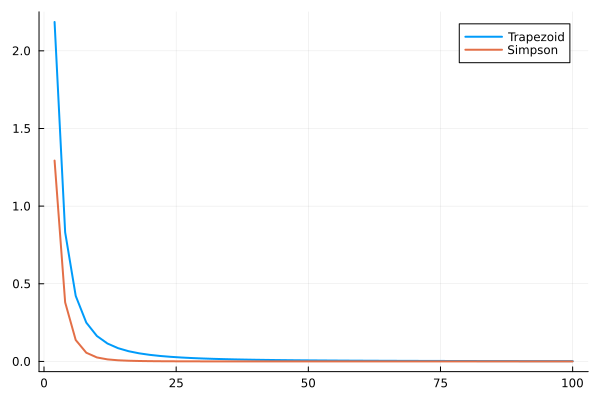
\includegraphics[scale=0.5]{plot_W1.png}
    \caption{Wykres błędu względnego aproksymacji całki z funkcji \(W_1(x)\).}
    \label{fig:plot_W1}
\end{figure}


\begin{figure}[h!]
    \centering
    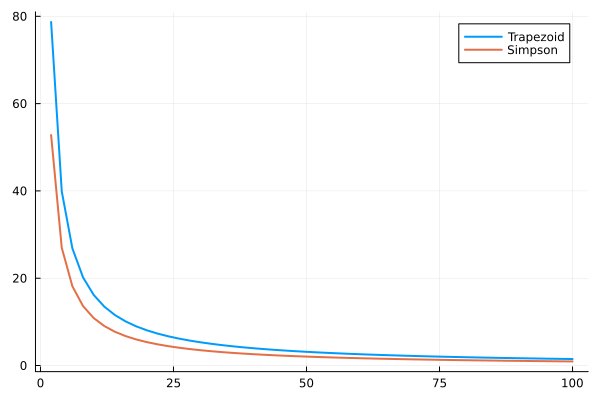
\includegraphics[scale=0.5]{plot_W2.png}
    \caption{Wykres błędu względnego aproksymacji całki z funkcji \(W_2(x)\).}
    \label{fig:plot_W2}
\end{figure}


\begin{figure}[h!]
    \centering
    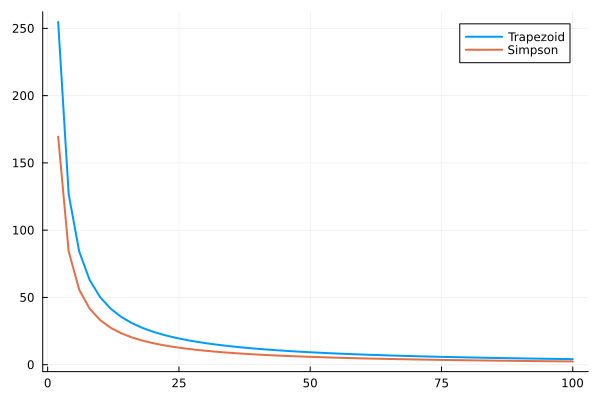
\includegraphics[scale=0.5]{plot_W3.png}
    \caption{Wykres błędu względnego aproksymacji całki z funkcji \(W_3(x)\).}
    \label{fig:plot_W3}
\end{figure}

\clearpage

\subsection{Funkcje wymierne}

Definiujemy

\begin{align*}
    P_1(x) &= \frac{1}{1+25x^2} \\
    P_2(x) &= \frac{(x-34)(x-398)(x-23)}{(x-230)(x+1,5)(x+7)(x+2)} \\
    P_3(x) &= \frac{1}{x^5 + x^4 + 3x^3 - 2x^2+7}
\end{align*}


\begin{figure}[h!]
    \centering
    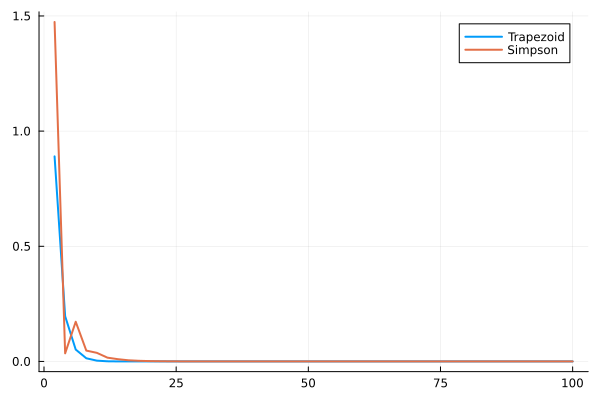
\includegraphics[scale=0.5]{plot_P1.png}
    \caption{Wykres błędu względnego aproksymacji całki z funkcji \(P_1(x)\).}
    \label{fig:plot_P1}
\end{figure}


\begin{figure}[h!]
    \centering
    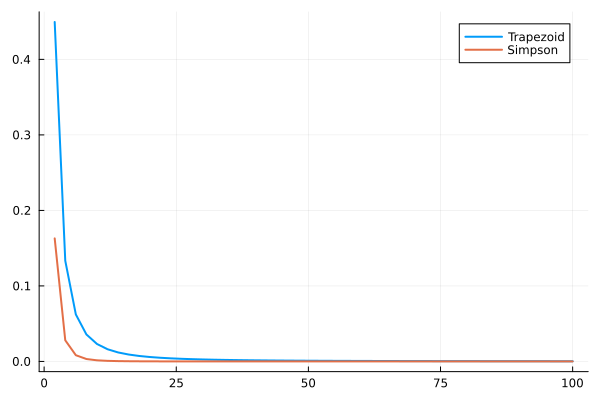
\includegraphics[scale=0.5]{plot_P2.png}
    \caption{Wykres błędu względnego aproksymacji całki z funkcji \(P_2(x)\).}
    \label{fig:plot_P2}
\end{figure}


\begin{figure}[h!]
    \centering
    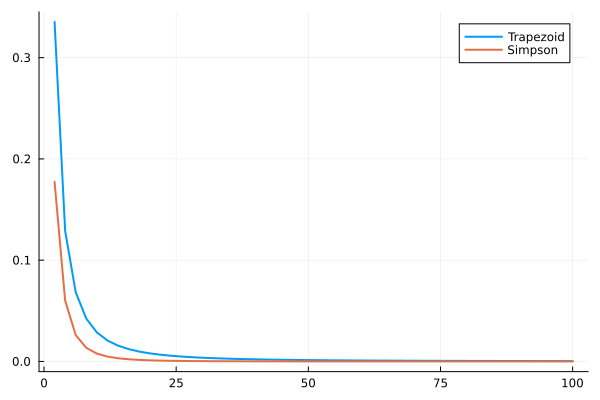
\includegraphics[scale=0.5]{plot_P3.png}
    \caption{Wykres błędu względnego aproksymacji całki z funkcji \(P_3(x)\).}
    \label{fig:plot_P3}
\end{figure}

\clearpage

\subsection{Funkcje wymierne złożone z funkcji trygonometrycznych}

Definiujemy

\begin{align*}
    T_1(x) &= \frac{\sin(x)}{\cos(x)^3 + 7} \\
    T_2(x) &= \frac{\sin(x)^2 + \cos(x)^5 + \sin(x)\cos(x) + 100}{\sin(x)^2\cos(x) + 8} \\
    T_3(x) &= \frac{\sin(x)}{\cos(x)^5+100}
\end{align*}


\begin{figure}[h!]
    \centering
    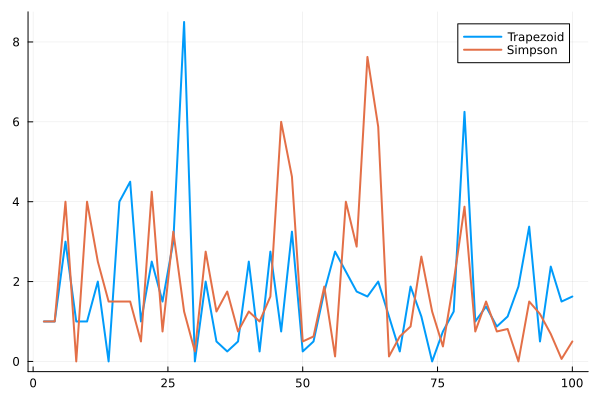
\includegraphics[scale=0.5]{plot_T1.png}
    \caption{Wykres błędu względnego aproksymacji całki z funkcji \(T_1(x)\).}
    \label{fig:plot_T1}
\end{figure}


\begin{figure}[h!]
    \centering
    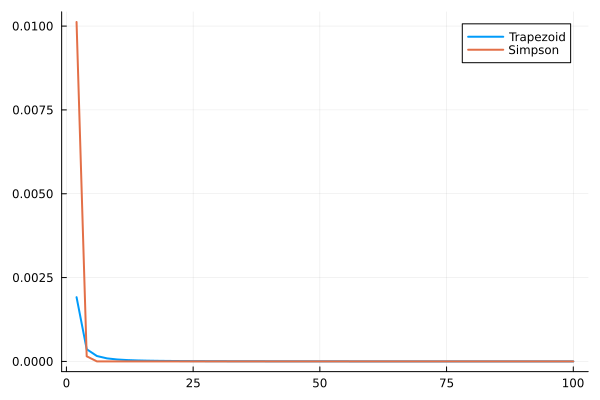
\includegraphics[scale=0.5]{plot_T2.png}
    \caption{Wykres błędu względnego aproksymacji całki z funkcji \(T_2(x)\).}
    \label{fig:plot_T2}
\end{figure}


\begin{figure}[h!]
    \centering
    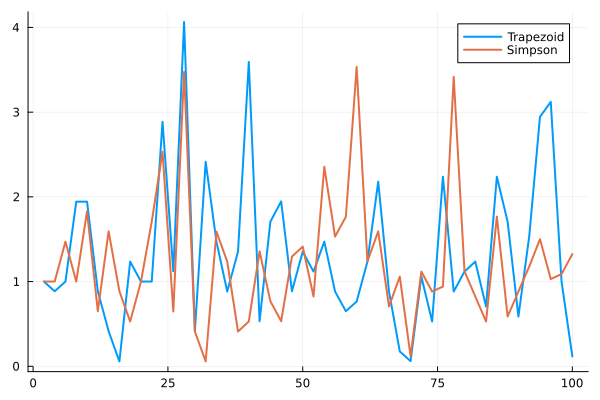
\includegraphics[scale=0.5]{plot_T3.png}
    \caption{Wykres błędu względnego aproksymacji całki z funkcji \(T_3(x)\).}
    \label{fig:plot_T3}
\end{figure}

\medskip

\noindent Można zauważyć, że wykresy \ref{fig:plot_T1} i \ref{fig:plot_T3} wyglądem odbiegają nieco od pozostałych. Dzieje się tak, ponieważ funkcje \(T_1(x)\) oraz \(T_3(x)\) są nieparzyste. Wobec tego całki z \(T_1\) oraz \(T_3\) na przedziale symetrycznym względem 0 są równe 0. Oczywiście przy ,,szczęśliwym'' doborze węzłów bardzo szybko uzyskamy wynik zbliżony do dokładnego.  Z drugiej strony przy obliczaniu kwadratur dla tych funkcji dodajemy liczby przeciwnych znaków bliskie sobie co do wartości bezwzględnej -- wobec tego występuje utrata cyfr znaczących. Oznacza to, że błąd względny, nawet przy dużej liczbie węzłów, może być duży. Można natomiast zauważyć (na wykresach \ref{fig:plot_T1_abs} oraz \ref{fig:plot_T3_abs}), że błąd bezwzględny jest mały -- mniejszy niż precyzja arytmetyki).


\begin{figure}[h!]
    \centering
    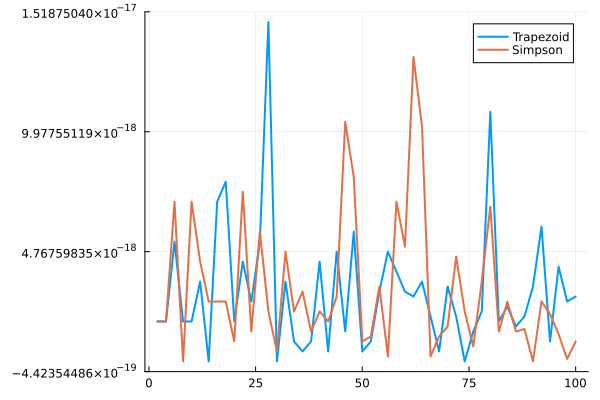
\includegraphics[scale=0.5]{plot_T1_abs.png}
    \caption{Wykres błędu bezwzględnego aproksymacji całki z funkcji \(T_1(x)\).}
    \label{fig:plot_T1_abs}
\end{figure}

\begin{figure}[h!]
    \centering
    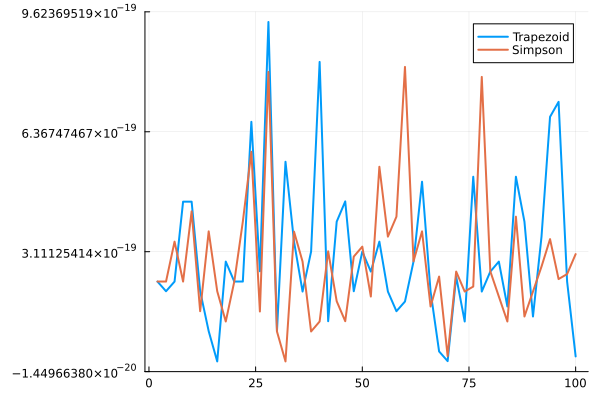
\includegraphics[scale=0.5]{plot_T3_abs.png}
    \caption{Wykres błędu bezwzględnego aproksymacji całki z funkcji \(T_3(x)\).}
    \label{fig:plot_T3_abs}
\end{figure}

\clearpage

% ----------------------------------------------------------------------
% -------------------- PORÓWNANIE CZASU OBLICZEŃ -----------------------
% ----------------------------------------------------------------------

\section{Porównanie czasu obliczeń}
\label{roz:czas}

W tej sekcji przedstawiam, jakie są najlepsze przybliżenia wartości błędu względnego aproksymacji całki dla metod trapezów i Simpsona przy ograniczeniu czasowym na obliczenia wykonywane przez program równym \( 0,001\) sekundy.

\begin{table}[!h]
    \centering
    \begin{tabular}{|c|c|c|}
            \hline
             Funkcja & Wzór trapezów &  Wzór Simpsona \\
             \hline \hline
            \(W_1\) & \(1,68701 \cdot 10^{-3} \) & \(3,08553 \cdot 10^{-6} \)\\
            \(W_2\) & 1,49043 & 0,94002 \\
            \(W_3\) & 35,53557 & 20,31242 \\
            \hline
    \end{tabular}
    \caption{Błędy względne dla funkcji wielomianowych.}
    \label{tab:wielomiany}
\end{table}


\begin{table}[!h]
    \centering
    \begin{tabular}{|c|c|c|}
            \hline
             Funkcja & Wzór trapezów &  Wzór Simpsona \\
             \hline \hline
            \(P_1\) &  \(8,97520 \cdot 10^{-6} \) & \(2.54633 \cdot 10^{-9}\) \\
            \(P_2\) &  \(2,35639 \cdot 10^{-4}\) & \(1,97046 \cdot 10^{-7}\) \\
            \(P_3\) &  \(3.36773 \cdot 10^{-4}\) & \(3.440313 \cdot 10^{-6}\) \\
            \hline
    \end{tabular}
    \caption{Błędy względne dla funkcji wymiernych.}
    \label{tab:wymierne}
\end{table}

\begin{table}[!h]
    \centering
    \begin{tabular}{|c|c|c|}
            \hline
             Funkcja & Wzór trapezów &  Wzór Simpsona \\
             \hline \hline
            \(T_1\) &  0 & 0 \\
            \(T_2\) &  \(5,84284 \cdot 10^{-7}\) & \(1,84524 \cdot 10^{-11}\) \\
            \(T_3\) &  0,05718 & 0,05718 \\
            \hline
    \end{tabular}
    \caption{Błędy względne dla funkcji wymiernych złożonych z funkcji trygonometrycznych.}
    \label{tab:trygonometryczne}
\end{table}

\noindent Można zatem zauważyć, że wzór Simpsona daje szybciej bardziej dokładne wyniki. 


% ----------------------------------------------------------------------
% ------------------------------ WNIOSKI -------------------------------
% ----------------------------------------------------------------------

\section{Wnioski}

Jak można zaobserwować na wykresach, wzór Simpsona daje dokładniejsze wyniki niż wzór trapezów dla takiej samej liczby węzłów. Ponadto, jak można zauważyć w tabelach \ref{tab:wielomiany}, \ref{tab:wymierne} oraz \ref{tab:trygonometryczne}, wzór Simpsona przy ograniczeniu czasowym w postaci \(0,001\) sekundy umożliwi nam poznanie dokładniejszych wyników niż wzór trapezów. W wynikach przeprowadzonych eksperymentów dostrzegamy więc przewagę wzoru Simpsona. 


\begin{thebibliography}{9}
\bibitem{kincaid}
David Kincaid, Ward Cheney, \emph{Analiza numeryczna}, Wydawnictwa Naukowo--Techniczne, 2005

\bibitem{nasa}
L. Richard Turner, \emph{Inverse of the Vandermonde matrix with applications}, National Aeronautics and Space Administration, 1966 
\end{thebibliography}

\end{document}
